\section{Results and Discussion} \label{sec:results_discussion}
This section presents the results of the security analysis and performance measurements, followed by a discussion of the findings.

\subsection{Security Analysis Results}
The effectiveness of VxLang virtualization was evaluated through static and dynamic analysis attempts to understand and bypass the authentication logic in the case study applications.

\subsubsection{Static Analysis (Ghidra)}
Static analysis of non-virtualized binaries using Ghidra was generally straightforward. Relevant strings (e.g., "Authentication Failed") and control flow for authentication logic were typically identifiable. For instance, in non-virtualized binaries, standard comparison instructions and conditional jumps controlling authentication were readily found (see Appendix Listings \ref{lst:asm_static_nonvirt_full}, \ref{lst:asm_static_cloud_full} in the full thesis for detailed examples), making static patching feasible.

Conversely, static analysis proved significantly more challenging for binaries processed by VxLang. Table \ref{tab:ghidra_summary_journal_en} summarizes key metrics from Ghidra analysis for representative applications, illustrating the impact of virtualization.

% --- ENGLISH: GHIDRA STATIC ANALYSIS SUMMARY TABLE (JOURNAL) ---
\begin{table}[!t]
    \centering
    \caption{Ghidra Static Analysis Metrics Comparison (Non-Virtualized vs. Virtualized)}
    \label{tab:ghidra_summary_journal_en}
    \resizebox{\columnwidth}{!}{%
    \begin{tabular}{@{}llrrrr@{}}
        \toprule
        \textbf{Application} & \textbf{Version} & \textbf{Instructions} & \textbf{Functions} & \textbf{Defined Data} & \textbf{Symbols} \\
        \midrule
        \multirow{3}{*}{app\_qt (GUI)} & Non-Virt. & 6104 & 538 & 1578 & 2113 \\
                                 \cmidrule(lr){2-6}
                                 & Virtualized & 214 & 25 & 174 & 103 \\
                                 \cmidrule(lr){2-6}
                                 & Change \% & \bo{-96.49\%} & \bo{-95.35\%} & \bo{-88.97\%} & \bo{-95.13\%} \\
        \midrule
        \multirow{3}{*}{console (CLI)} & Non-Virt. & 3090 & 261 & 726 & 1018 \\
                                 \cmidrule(lr){2-6}
                                 & Virtualized & 174 & 20 & 146 & 88 \\
                                 \cmidrule(lr){2-6}
                                 & Change \% & \bo{-94.37\%} & \bo{-92.34\%} & \bo{-79.89\%} & \bo{-91.36\%} \\
        \midrule
        \multirow{3}{*}{encryption (Benchmark)} & Non-Virt. & 6282 & 368 & 849 & 1920 \\
                                 \cmidrule(lr){2-6}
                                 & Virtualized & 159 & 20 & 155 & 77 \\
                                 \cmidrule(lr){2-6}
                                 & Change \% & \bo{-97.47\%} & \bo{-94.57\%} & \bo{-81.74\%} & \bo{-95.99\%} \\
        \bottomrule
    \end{tabular}%
    }
\end{table}
% --- END ENGLISH: GHIDRA STATIC ANALYSIS SUMMARY TABLE (JOURNAL) ---

The data in Table \ref{tab:ghidra_summary_journal_en} consistently shows a drastic reduction (typically >90\%) in the number of recognizable instructions, functions, defined data, and symbols in virtualized binaries. For instance, the \texttt{app\_qt} application saw its recognizable instructions decrease from 6104 to 214 (a \bo{-96.49\%} change) and functions from 538 to 25 (a \bo{-95.35\%} change) after virtualization. This starkly contrasts with non-virtualized versions, indicating a fundamental transformation of the code into a format uninterpretable by standard disassembly. This reduction in identifiable program elements severely impedes static analysis, making it nearly impossible to locate and comprehend the relevant control flow logic for authentication or other critical functions. Static bypass attempts on virtualized binaries were consequently unsuccessful. These findings align with the understanding that static disassemblers struggle with custom bytecode ISAs introduced by virtualization \cite{Sikorski2012, Eilam2011, Ko2007}. The file size also increased substantially (e.g., \texttt{app\_qt.exe} from 122 KB to 1,578 KB after virtualization, a ~13x increase), indicative of the embedded VM and bytecode.

\subsubsection{Dynamic Analysis (x64dbg)}
Dynamic analysis of non-virtualized binaries using x64dbg was generally straightforward. Setting breakpoints based on string references or near conditional jumps identified during static analysis proved effective. Stepping through the code clearly revealed comparison logic and conditional jumps, and runtime patching successfully bypassed authentication.

For VxLang-virtualized binaries, dynamic analysis presented a more nuanced challenge, as summarized by key metrics in Table \ref{tab:x64dbg_summary_journal_en}.

% --- ENGLISH: X64DBG DYNAMIC ANALYSIS SUMMARY TABLE (JOURNAL) ---
\begin{table}[!t]
    \centering
    \caption{x64dbg Dynamic Analysis Metrics Comparison (Non-Virtualized vs. Virtualized)}
    \label{tab:x64dbg_summary_journal_en}
    \resizebox{\columnwidth}{!}{%
    \begin{tabular}{@{}llrrrl@{}}
        \toprule
        \textbf{Application} & \textbf{Version} & \textbf{Instr. Count (Observed)} & \textbf{Mem. Sections} & \textbf{Def. Symbols} & \textbf{Key Str. Found} \\
        \midrule
        \multirow{3}{*}{app\_qt (GUI)} & Non-VM & 8022 & 7 & 209 & Yes \\
                                 \cmidrule(lr){2-6}
                                 & VM & 8011 & 10 & 15 & No \\
                                 \cmidrule(lr){2-6}
                                 & Change \% & -0.14\% & +42.86\% & \bo{-92.82\%} & - \\
        \midrule
        \multirow{3}{*}{console (CLI)} & Non-VM & 5797 & 6 & 88 & Yes \\
                                 \cmidrule(lr){2-6}
                                 & VM & 5843 & 9 & 12 & No \\
                                 \cmidrule(lr){2-6}
                                 & Change \% & +0.79\% & +50.00\% & \bo{-86.36\%} & - \\
        \midrule
        \multirow{3}{*}{encryption (Benchmark)} & Non-VM & 8336 & 6 & 94 & Yes \\
                                 \cmidrule(lr){2-6}
                                 & VM & 8207 & 9 & 13 & No \\
                                 \cmidrule(lr){2-6}
                                 & Change \% & -1.55\% & +50.00\% & \bo{-86.17\%} & - \\
        \bottomrule
    \end{tabular}%
    }
\end{table}
% --- END ENGLISH: X64DBG DYNAMIC ANALYSIS SUMMARY TABLE (JOURNAL) ---

Key observations from dynamic analysis of virtualized binaries include:
\begin{itemize}
    \item \textbf{Visibility of Native VM Instructions:} Once the virtualized application was fully loaded, x64dbg displayed valid native x86-64 instructions. These instructions belong to the VxLang VM interpreter, not the original application's native logic. The observed instruction count (Table \ref{tab:x64dbg_summary_journal_en}) did not drastically change, reflecting VM activity rather than revealing the original program's complexity to the analyst.
    \item \textbf{Increased Memory Sections:} The number of memory sections consistently increased (by 40-50\%), likely due to the VxLang runtime and bytecode.
    \item \textbf{Persistent Obscurity of Critical Data and Application Logic:}
        \begin{itemize}
            \item \textbf{Key String Obfuscation:} Critical strings targeted for virtualization (e.g., "Authentication Failed") were \textbf{not found} using standard runtime searches in x64dbg (Table \ref{tab:x64dbg_summary_journal_en}, "Key Str. Found": No). This demonstrates effective runtime string protection.
            \item \textbf{Drastic Reduction in Defined Symbols:} Observable defined symbols were significantly reduced (by >85\%), hampering contextual understanding and navigation.
            \item \textbf{Abstraction of Application Logic:} The core application logic was transformed into internal bytecode executed by the VxLang VM. Debuggers show the VM's execution, not the direct native execution of the original logic, making it extremely difficult to trace or understand the application's intended behavior.
        \end{itemize}
    \item \textbf{Ineffectiveness of Simple Runtime Patching:} Consequently, attempts to bypass authentication by patching simple conditional jumps at runtime were rendered ineffective. The critical decision-making points were embedded within the VM's opaque execution flow.
\end{itemize}
These dynamic analysis findings align with the principles of VM-based obfuscation \cite{Sikorski2012, Ore06}. While the debugger can step through the VM interpreter's native code, the actual application logic is abstracted away, making direct analysis and manipulation exceptionally difficult without deep knowledge of the VM's architecture \cite{Sal18}.

\subsubsection{Analysis of Potentially Malicious Software and VirusTotal Detection}
To evaluate VxLang's impact on more complex software and automated detection, ten software samples, including the Lilith RAT client \cite{LilithRAT} and nine other publicly available malware/PUA samples (\textit{Al-Khaser, donut, DripLoader, FilelessPELoader, JuicyPotato, ParadoxiaClient, PELoader, RunPE-In-Memory, SigLoader}), were analyzed. For the Lilith RAT, after careful, iterative placement of VxLang macros targeting critical functions, functional testing confirmed that the virtualized client remained fully operational, successfully connecting to its server and executing remote commands. This demonstrated VxLang's capability to preserve core functionalities in complex applications if applied precisely.

All ten samples, in their original and VxLang-virtualized forms, were submitted to VirusTotal (72 AV engines). The results showed a varied impact on detection rates. For five samples, including Lilith RAT (22 to 18 detections) and \textit{donut} (30 to 19 detections), virtualization led to a decrease in detections, often accompanied by a shift from specific threat labels to more generic ones or AI/heuristic-based flags. This suggests successful obfuscation of static signatures.

However, for the other five samples, such as \textit{JuicyPotato} (9 to 20 detections) and \textit{FilelessPELoader} (16 to 21 detections), virtualization resulted in an \textit{increase} in detections. This indicates that the virtualization layer itself or its artifacts can trigger suspicion from some AV engines, potentially being flagged as packed or protected software common in malware. Overall, the average change in detection across all ten samples was minimal (+0.4 detections), highlighting that while VxLang can alter detection profiles, it does not guarantee evasion and its effect is sample-dependent. Detailed per-sample detection counts are available in the extended thesis work.

\subsection{Performance and Size Overhead Results}

\subsubsection{Execution Time Overhead}
The performance impact was measured using QuickSort and AES benchmarks.

\begin{itemize}
	\item \textbf{QuickSort:} As shown in Table \ref{tab:quick_sort_performance_journal} and Fig. \ref{fig:quick_sort_performance_journal}, virtualization introduced substantial execution time overhead. The overhead increased with data size, ranging from approximately 27,300\% for 100 elements (0.01 ms to 2.74 ms) to about 15,150\% for 1,000,000 elements (218.32 ms to 33,292.91 ms). This indicates a significant constant overhead plus a scaling factor imposed by the VM's interpretation loop for the recursive sorting function.
	      \begin{table}[!t]
		      \centering
		      \caption{Quick Sort Execution Time Results (ms)}
		      \label{tab:quick_sort_performance_journal}
		      \resizebox{\columnwidth}{!}{%
			      \begin{tabular}{@{}lrrrr@{}}
				      \toprule
				      \multirow{2}{*}{\textbf{Array Size}} & \multicolumn{2}{c}{\textbf{Non-Virtualized}} & \multicolumn{2}{c}{\textbf{Virtualized}}                                        \\
				      \cmidrule(lr){2-3} \cmidrule(lr){4-5}
				                                           & \textbf{Avg Time}                            & \textbf{Std Dev}                         & \textbf{Avg Time} & \textbf{Std Dev} \\
				      \midrule
				      100                                  & 0.01                                         & 0.00                                     & 2.74              & 0.38             \\
				      1,000                                & 0.08                                         & 0.00                                     & 27.35             & 1.25             \\
				      5,000                                & 0.54                                         & 0.05                                     & 144.44            & 8.25             \\
				      10,000                               & 1.24                                         & 0.08                                     & 295.77            & 13.68            \\
				      50,000                               & 6.98                                         & 0.51                                     & 1,556.15          & 122.81           \\
				      100,000                              & 15.12                                        & 1.26                                     & 3,080.30          & 303.02           \\
				      500,000                              & 104.44                                       & 7.30                                     & 14,298.92         & 374.98           \\
				      1,000,000                            & 218.32                                       & 8.10                                     & 33,292.91         & 4,342.93         \\
				      \bottomrule
			      \end{tabular}
		      } % End resizebox
	      \end{table}

	      \begin{figure}[!t]
		      \centering
		      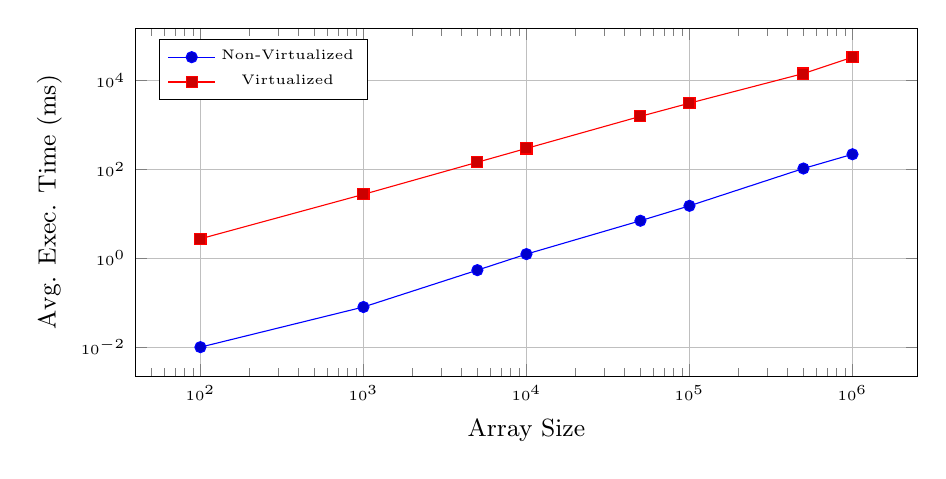
\begin{tikzpicture}
			      \begin{axis}[
					      width=0.95\columnwidth,
					      height=6cm,
					      xlabel={Array Size},
					      ylabel={Avg. Exec. Time (ms)},
					      xmode=log,
					      log basis x={10},
					      ymode=log,
					      log basis y={10},
					      legend pos=north west,
					      grid=major,
					      tick label style={font=\tiny},
					      label style={font=\small},
					      legend style={font=\tiny}
				      ]
				      \addplot coordinates {
						      (100, 0.01)
						      (1000, 0.08)
						      (5000, 0.54)
						      (10000, 1.24)
						      (50000, 6.98)
						      (100000, 15.12)
						      (500000, 104.44)
						      (1000000, 218.32)
					      };
				      \addlegendentry{Non-Virtualized};

				      \addplot coordinates {
						      (100, 2.74)
						      (1000, 27.35)
						      (5000, 144.44)
						      (10000, 295.77)
						      (50000, 1556.15)
						      (100000, 3080.30)
						      (500000, 14298.92)
						      (1000000, 33292.91)
					      };
				      \addlegendentry{Virtualized};
			      \end{axis}
		      \end{tikzpicture}
		      \caption{Quick Sort Execution Time Comparison (Log-Log Scale).}
		      \label{fig:quick_sort_performance_journal}
	      \end{figure}


	\item \textbf{AES Encryption:} Table \ref{tab:aes_performance_journal} shows that the total time for encrypting 976MB of data increased by approximately 396.7\% (1878.52 ms to 9330.73 ms), and decryption time increased by about 562.9\% (1304.75 ms to 8649.74 ms). Consequently, the combined throughput dropped dramatically from 634.16 MB/s to 108.78 MB/s (an 82.8\% reduction). This confirms a significant overhead for cryptographic operations.
	      \begin{table}[!t]
		      \centering
		      \caption{AES-256-CBC Performance Results (976MB Data)}
		      \label{tab:aes_performance_journal}
		      \resizebox{\columnwidth}{!}{%
			      \begin{tabular}{@{}lrr@{}}
				      \toprule
				      \textbf{Metric}              & \textbf{Non-Virtualized} & \textbf{Virtualized} \\
				      \midrule
				      Total Encryption Time (ms)   & 1,878.52                 & 9,330.73             \\
				      Total Decryption Time (ms)   & 1,304.75                 & 8,649.74             \\
				      Avg. Encrypt Time/Block (ms) & 0.00188                  & 0.00933              \\
				      Avg. Decrypt Time/Block (ms) & 0.00130                  & 0.00865              \\
				      Encrypt Throughput (MB/s)    & 519.86                   & 104.66               \\
				      Decrypt Throughput (MB/s)    & 748.46                   & 112.90               \\
				      Combined Throughput (MB/s)   & 634.16                   & 108.78               \\
				      \bottomrule
			      \end{tabular}
		      } % End resizebox
	      \end{table}

\end{itemize}

\subsubsection{File Size Overhead}
Table \ref{tab:file_size_journal} shows a consistent increase in executable file size after virtualization. For smaller console/benchmark programs (\texttt{quick\_sort}, \texttt{encryption}, \texttt{console}, \texttt{Lilith\_Client}), the size increased by over 15-18 times (from ~80-110 KB to ~1.5-1.6 MB). For larger GUI applications (\texttt{app\_imgui} from 1,675 KB to 2,330 KB; \texttt{app\_qt} from 122 KB to 1,578 KB) and the benchmark with embedded data (\texttt{size} from 97,771 KB to 112,324 KB), the relative increase was smaller but still significant. This overhead is primarily attributed to the inclusion of the VxLang VM runtime and the bytecode representation of the original code.
\begin{table}[H]
	\centering
	\caption{Executable File Size Comparison (KB)}
	\label{tab:file_size_journal}
	\resizebox{\columnwidth}{!}{
		\begin{tabular}{@{}lrr@{}}
			\toprule
			\textbf{Program}  & \textbf{Non-Virtualized (KB)} & \textbf{Virtualized (KB)} \\
			\midrule
			quick\_sort       & 98                            & 1,537                     \\
			encryption        & 110                           & 1,507                     \\
			size              & 97,771                        & 112,324                   \\
			console           & 92                            & 1,577                     \\
			console\_cloud    & 281                           & 1,695                     \\
			app\_imgui        & 1,675                         & 2,330                     \\
			app\_imgui\_cloud & 1,860                         & 2,418                     \\
			app\_qt           & 122                           & 1,578                     \\
			app\_qt\_cloud    & 315                           & 1,671                     \\
			Lilith\_Client    & 84                            & 1,554                     \\
			\bottomrule
		\end{tabular}
	}
\end{table}

\subsection{Discussion}
The experimental results clearly demonstrate the core trade-off inherent in using VxLang's code virtualization.

\textbf{Security Enhancement and Detection Evasion:} VxLang provides a substantial barrier against common reverse engineering techniques. The transformation into interpreted bytecode neutralizes standard static analysis tools like Ghidra, which rely on recognizable native instruction patterns \cite{Eilam2011, Ko2007}, and significantly complicates dynamic analysis with tools like x64dbg, as the underlying logic is executed by an opaque VM \cite{Sikorski2012}. This aligns with the established understanding that VM-based obfuscation fundamentally alters the code structure beyond the interpretation capabilities of standard disassemblers \cite{Ore06, Sal18}. Furthermore, the VirusTotal analysis on ten malware/PUA samples revealed a nuanced impact: while VxLang could reduce signature-based detections for some samples, it led to increased detections for others, likely due to the virtualization layer itself being flagged. This highlights a complex interplay between obfuscation and evolving AV detection heuristics \cite{Ore06, Sal18, Rou13}.

\textbf{Performance Cost:} The security and evasion benefits come at a steep price in terms of performance. The interpretation overhead significantly slows down virtualized code, especially for computationally intensive tasks (QuickSort overhead of ~15,000\% for 1M elements; AES throughput reduction of ~83\%), potentially rendering indiscriminate application impractical due to severe speed degradation.

\textbf{Size Increase:} The considerable increase in file size (e.g., 15-18x for small applications), mainly due to the embedded VM runtime, is another factor, particularly relevant for smaller applications or distribution constraints.

\textbf{Practical Implications:} VxLang appears potent for protecting highly sensitive code where security and potentially detection evasion are paramount, and the performance impact on those specific segments is acceptable (e.g., anti-tamper, licensing, core IP). The Lilith case shows it can protect complex logic without breaking it. However, the severe performance cost necessitates a strategic, selective application, targeting only critical sections. The VirusTotal results also imply that while detection profiles are altered, evasion is not guaranteed, as heuristic/AI methods or flags for protected software can still lead to detection, and in some cases, increase it. The choice between hardcoded and cloud-based authentication showed that protecting client-side logic handling the result of validation remains crucial, reinforcing the need for techniques like virtualization on critical checks, regardless of where primary authentication occurs.
